
\documentclass[a4paper, landscape]{article}
\usepackage[margin=1.5cm]{geometry}
\usepackage{fontspec}
\setmainfont{Latin Modern Roman}
\setmonofont{DejaVu Sans Mono}

\usepackage{graphicx}
\usepackage{xcolor}
\usepackage{listings}
\usepackage{hyperref}
\usepackage{tabularx} % For tables that fit the page width
\usepackage{multirow} % For cells that span multiple rows

\lstset{
    basicstyle=\ttfamily\small,
    breaklines=true,
}

\begin{document}
\title{Simulation Run Summary}
\author{Contiki-NG RPL Project}
\maketitle


% --- Entry for simulation 20250818124554 ---
\begin{tabularx}{\textwidth}{|l|X|X|X|m{5.5cm}|}
\hline
\textbf{Start} & \textbf{Sim Run} & \textbf{Source File} & \multicolumn{2}{c|}{\textbf{DODAG 1 Graph}} \\
\texttt{GMT+1200} & \texttt{20250818124554} & \texttt{text\_20250818124554.txt} & \multicolumn{2}{c|}{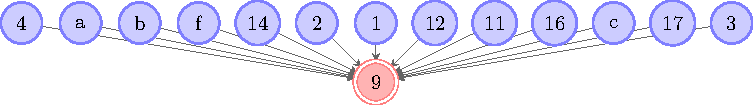
\includegraphics[page=1, height=2.5cm, keepaspectratio]{/home/stevecos/data/graph_20250818124554.pdf}} \\
\hline
\textbf{Finish} & \textbf{MOP} & \textbf{OFs} & \multicolumn{2}{c|}{\textbf{DODAG 2 Graph}} \\
\texttt{18 Aug 12:48} & \texttt{N/A} & \texttt{N/A} & \multicolumn{2}{c|}{\includegraphics[page=2, height=2.5cm, keepaspectratio]{/home/stevecos/data/graph_20250818124554.pdf}} \\
\hline
\textbf{Notes} & \multicolumn{4}{l|}{} \\ % Empty notes cell spanning 4 columns
\hline
\end{tabularx}
\vspace{1cm}

\end{document}
